\subsection{Base de données}
La base de données d'images que nous avons utilisé est la base AT\&T\\
(lien : \url{http://www.cl.cam.ac.uk/research/dtg/attarchive/facedatabase.html}).
C'est une base de 400 images de visages de 40 personnes, avec 10 images 
par personne. Les visages sont bien centrés sur l'image et l'arrière-plan
est très peu apparent ; ça correspond au genre d'images obtenues après une étape de 
détection (localisation) de visage. La figure \ref{fig:implementation:bdd_exemple} montre
un échantillon des images de la base.
\begin{figure}[H]
    \centering
    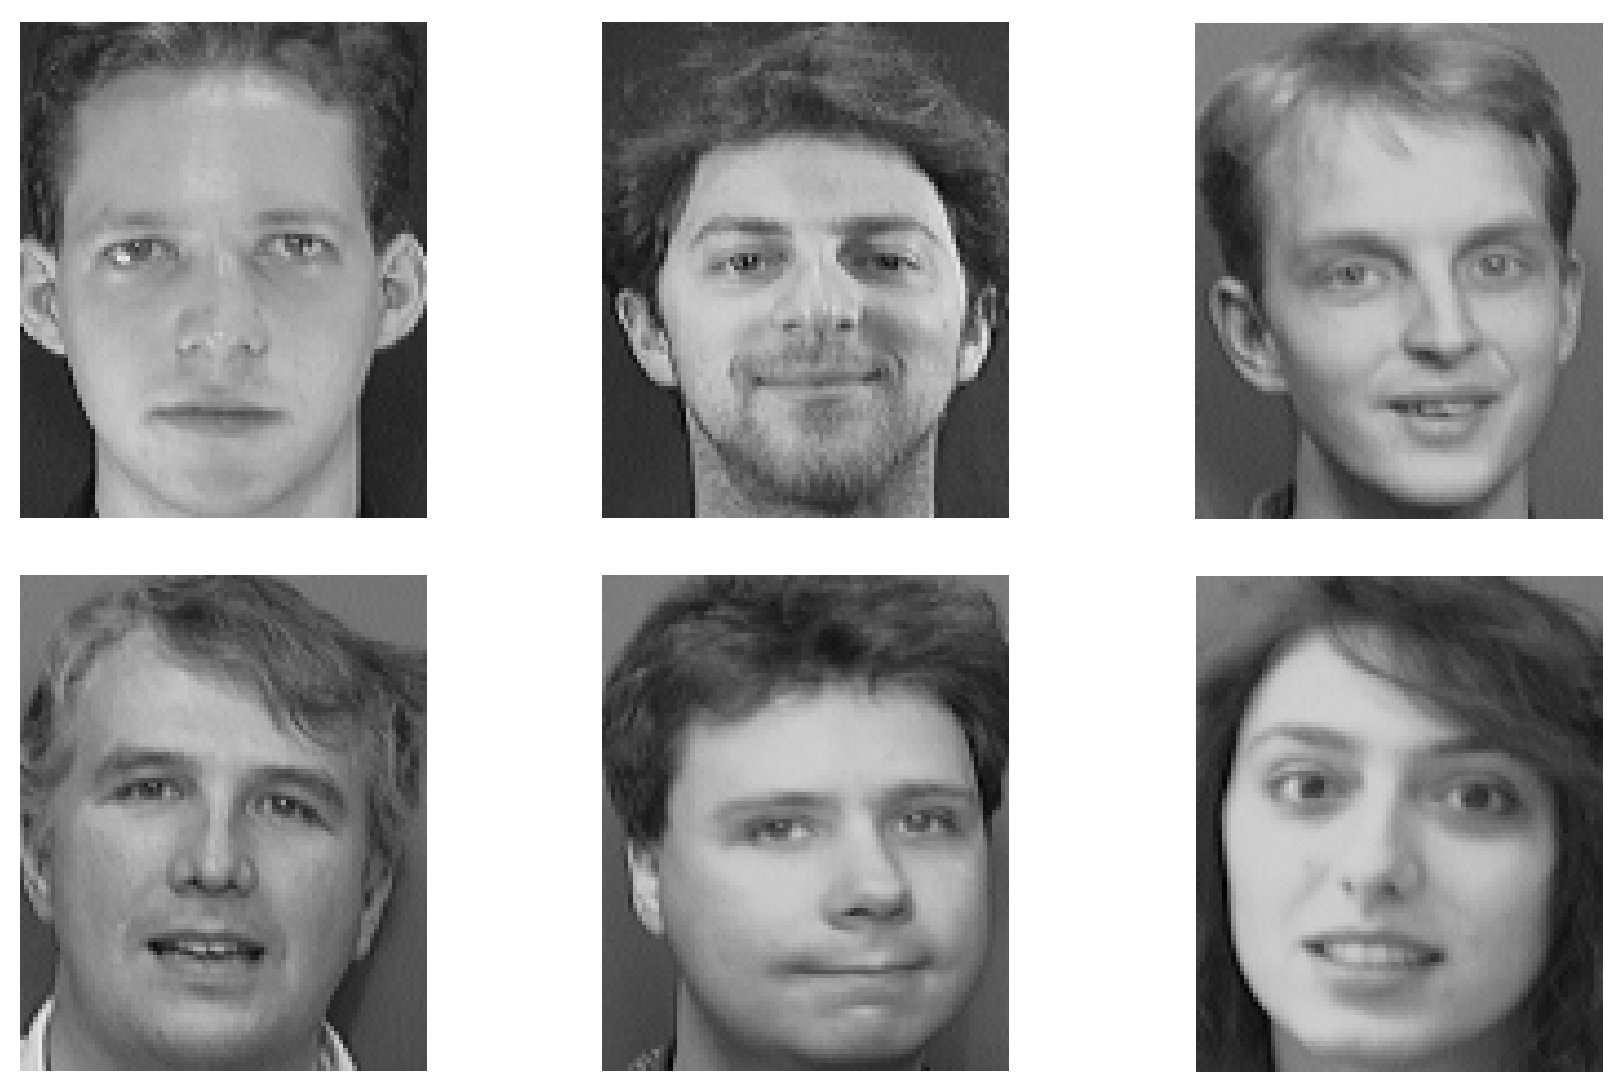
\includegraphics[scale=0.4]{images/bdd_exemple}
    \caption{Échantillon des images de la base de données AT\&T.}
    \label{fig:implementation:bdd_exemple}
\end{figure}
Les images sont en niveaux de gris et ont une taille de $92 \times 112$.


\subsection{Méthodologie de test}
Étant donné que nous avons un nombre limité d'images, nous ne pouvons pas
nous permettre de partitionner l'ensemble des 400 images en données 
d’entraînement et de test ; la variance des résultats obtenus les rendrait
inexploitable (à vrai dire on a essayé ça, le taux de classification correcte
varie entre $50\%$ et $80\%$ pour deux choix aléatoires des données d'entraînement
et de test, ce qui est une marge trop large).

Pour tester les performances du système, nous allons utiliser la validation croisée.
La validation croisée est une méthode d’estimation des performances d'un algorithme
d'apprentissage automatique. On divise l'ensemble des images en $k$ échantillons, 
puis on sélectionne un des $k$ échantillons comme ensemble de test et les $k-1$ autres
échantillons comme ensemble d'apprentissage. On apprend le modèle sur
l'ensemble d'apprentissage et on mesure le taux de classification correcte sur l'ensemble
de test. On répète l'opération en sélectionnant un autre échantillon de test parmi les $k-1$
échantillons qui n'ont pas encore été utilisés pour tester le modèle. 
L'opération se répète ainsi $k$ fois pour de sorte que chaque sous-échantillon ait été utilisé exactement
une fois comme ensemble de test. La moyenne des $k$ taux de classification correcte servira
d'estimation finale du taux de classification correcte du système.

Dans notre cas, nous avons pris $k = 10$. Pour chaque personne,
9 images d'entraînement et une de test pour chaque itération.
À noter que contrairement à ce qui a été fait dans \cite{article},
les eigenfaces ont été calculées en utilisant uniquement les données
d'entraînement, ce qui permet d'avoir une estimation plus correcte 
des performances du système.


\subsection{Résultats obtenus}
Nous avons obtenu un taux de reconnaissance correcte de $68\%$, ce qui est proche
du taux obtenu par \cite{article} sans normalisation des eigenfaces (à savoir $70\%$).
Notre taux de $68\%$ a été obtenu en normalisant les eigenfaces, cette normalisation
n'influence que très peu le taux de reconnaissance.

Il est à mentionner que nous avons travaillé avec 40 classes, et \cite{article}
ont travaillé avec 20 classes. Quand nous réduisons le nombre de classes à 20
(et donc le nombre d'images à 200), nous obtenons un taux de reconnaissance
correcte de $82\%$, ce qui est assez proche du taux de $89.5\%$ obtenu par \cite{article}.